\documentclass{article}
\usepackage{color}
\usepackage{listings}
\usepackage{graphicx}
\usepackage{subfig}
\usepackage{caption}
\usepackage{subcaption}
\usepackage{amsmath}
\usepackage{cite}
\usepackage{url}
\usepackage{setspace,lipsum}% http://ctan.org/pkg/{setspace,lipsum}

\lstset{ %
language=java,                % choose the language of the code
basicstyle=\footnotesize,       % the size of the fonts that are used for the code
numbers=left,                   % where to put the line-numbers
numberstyle=\footnotesize,      % the size of the fonts that are used for the line-numbers
stepnumber=1,                   % the step between two line-numbers. If it is 1 each line will be numbered
numbersep=5pt,                  % how far the line-numbers are from the code
backgroundcolor=\color{white},  % choose the background color. You must add \usepackage{color}
showspaces=false,               % show spaces adding particular underscores
showstringspaces=false,         % underline spaces within strings
showtabs=false,                 % show tabs within strings adding particular underscores
frame=single,           % adds a frame around the code
tabsize=2,          % sets default tabsize to 2 spaces
captionpos=b,           % sets the caption-position to bottom
breaklines=true,        % sets automatic line breaking
breakatwhitespace=false,    % sets if automatic breaks should only happen at whitespace
escapeinside={\%*}{*}          % if you want to add a comment within your code
}

% Informationen ------------------------------------------------------------
% 	Definition von globalen Parametern, die im gesamten Dokument verwendet
% 	werden können (z.B auf dem Deckblatt etc.).
% --------------------------------------------------------------------------
\newcommand{\titel}{Ermittlung des stationären Zustands beim Festplattenbenchmarking}
\newcommand{\art}{Exposé} %Bachelorarbeit
\newcommand{\ort}{Leipzig}
\newcommand{\hochschule}{Universität Leipzig}
\newcommand{\fachgebiet}{Abteilung Datenbanken}
\newcommand{\fakultaet}{Fakultät für Mathematik und Informatik}
\newcommand{\institut}{Institut für Informatik}
\newcommand{\autor}{xxxx xxxxx}
\newcommand{\matrikelnr}{xxxxxxx}
\newcommand{\erstbetreuer}{Prof. Dr. Erhard Rahm}
\newcommand{\zweitbetreuer}{XXXXX}
\newcommand{\jahr}{xxxx}
\newcommand{\invnr}{1337}
\newcommand{\eingereicht}{xx.xx.xxxx}

% Eigene Befehle
\newcommand{\todo}[1]{\textbf{\textsc{\textcolor{red}{(TODO: #1)}}}}

% Autorennamen in small caps
\newcommand{\AutorZ}[1]{\textsc{#1}}
\newcommand{\Autor}[1]{\AutorZ{\citeauthor{#1}}}

% Befehle zur semantischen Auszeichnung von Text
\newcommand{\NeuerBegriff}[1]{\textbf{#1}}
\newcommand{\Fachbegriff}[1]{\textit{#1}}
\newcommand{\Prozess}[1]{\textit{#1}}
\newcommand{\Webservice}[1]{\textit{#1}}
\newcommand{\Eingabe}[1]{\texttt{#1}}
\newcommand{\Code}[1]{\texttt{#1}}
\newcommand{\Datei}[1]{\texttt{#1}}
\newcommand{\Datentyp}[1]{\textsf{#1}}
\newcommand{\XMLElement}[1]{\textsf{#1}}

% Abkürzungen
\newcommand{\vgl}{Vgl.\ }
\newcommand{\ua}{\mbox{u.\,a.\ }}
\newcommand{\zB}{\mbox{z.\,B.\ }}
\newcommand{\bs}{$\backslash$}

% Einfache Anführungszeichen in texttt
\newcommand{\sq}{\textquotesingle}


\begin{document}

\thispagestyle{plain}
\begin{titlepage}

\begin{center}

\institut\\
\fakultaet\\
\fachgebiet\\[6ex]

\textbf{\large\titel}\\[1.5ex]
\art\\[6ex]

\normalsize
vorgelegt von:\\
\autor\\[1.5ex]
Matrikelnummer:\\
\matrikelnr\\[1.5ex]
Betreuer:\\
\erstbetreuer\\
\zweitbetreuer\\[1.0ex]
\end{center}

%\begin{tabbing}
%\hspace{3.5cm}\= \kill
%   vorgelegt von: \> \autor\\[1.2ex]
%   Matrikelnummer: \> \matrikelnr\\[1.2ex]
%    \> \\
%   Betreuer: \> \erstbetreuer\\[1.2ex]
%    \> \zweitbetreuer
%\end{tabbing}

\begin{center}
\copyright\ \jahr\\[1.0ex]
\end{center}

\singlespacing
\small
\noindent Dieses Werk einschließlich seiner Teile ist \textbf{urheberrechtlich geschützt}. Jede Verwertung außerhalb der engen Grenzen des Urheberrechtgesetzes ist ohne Zustimmung des Autors unzulässig und strafbar. Das gilt insbesondere für Vervielfältigungen, Übersetzungen, Mikroverfilmungen sowie die Einspeicherung und Verarbeitung in elektronischen Systemen.



\end{titlepage}


\tableofcontents{}


\newpage

\begin{abstract}
Mit Benchmarks kann man die Performanz von Computersystemen, wie etwa die Rechenleistung und die I/O-Geschwindigkeit messen. Diese Messungen können stark oder schwach schwanken, je nachdem, ob ein Warm-Up erfolgte. Für die Ermittlung des stationären Zustandes sind geringe Schwankungen bei den Messungen notwendig. In dieser Arbeit wird mit dem Benchmark-Tool Fio gearbeitet, und es wird ein Analysetool entwickelt, das diesen Zustand ermittelt. Dabei wird statistische Analyse angewendet, um diesen stationären Zustand zu bestimmen. Das Programm wird in Java geschrieben.

\end{abstract}

\newpage
\section{Einführung}
Die Performanz eines Rechners ist die Leistungsfähigkeit und Effizienz bei der Ausführung von Aufgaben \cite{Delst}. Um herauszufinden welche Rechner die beste Performanz liefert, sind Messungen notwendig, um sie vergleichen zu können. Diese Messungen und Vergleiche werden mit Benchmarks durchgeführt \cite{takevalue}.
Mit ihnen wird die Rechenleistung oder auch Lese-/Schreibgeschwingkeit der Hardware oder auch Software mit standardisierten Tests gemessen \cite{benchmarkingBruno2014}. Ein Beispiel, bei dem Software getestet wird, sind virtuelle Maschinen wie die Java Virtual Machine \cite{10.1145/1297027.1297033} oder virtuelle Maschinen die auf reale Rechner basieren.
Hier wird die Performanz von virtuellen CPUs oder des Hypervisor analysiert \cite{9256518}.
Auch für Cloud Computing Platformen wird Benchmarking betrieben, um auch Performanz zwischen verschieden Cloudplatformen vergleichen zu können. Diese Benchmarks verwenden z.B die Turnaround-Zeit als Metrik, also die Zeit, die ein Prozess benötigt, um vollständig durchzulaufen \cite{10.1145/2493123.2462919}.  Somit gibt es ein weites Spektrum an Auswahl von Systemen, wo  Benchmarking betrieben wird.
Solche Grenzen könnten die Hardware (z. B. CPU-Taktrate oder Bandbreitengeschwindigkeit beim Lesen oder Schreiben), aber auch Software (Virtuelle Maschinen) sein.
Und mit der Verbesserung von solchen Speichermedien, wie HDD zu SSD, und CPU-Leistung wird die I/O Geschwindigkeit immer relevanter. Studien haben schon bewiesen, dass dies eine Ursache für Bottlenecks in der Performanz ist \cite{analysisNVMeSSD}.

In Großkonzernen sind oft Performanzprobleme die eigentlichen Hindernisse, und nicht die funktionalen Probleme. Serviceausfälle sind höchst kostspielig und sollten minimiert werden \cite{whenStopPerformanceTest}. 

Ein Beispielprogramm für so ein Benchmark Tool ist das Fio (flexible I/O tester) \cite{axboe2021github}.
Fio ist ein Tool, mit dem man die Bandbreitengeschwindigkeit vom Lesen/Schreiben testet und sie als eine Textdatei (von fio Logdatei genannt) ausgeben kann. Diese Geschwindigkeit kann stärker oder schwächer vom eigentlichen WERT schwanken. Das Ziel meines Tools ist es, den stationären Zustand zu ermitteln.
Ein Zustand, wo die Rechenleistung oder Lese-/Schreibgeschwindigkeit sich nicht mehr beim Messen stark ändert \cite{vmsHotandCold}. 
Um den stationären Zustand zu ermitteln, werden verschiedene Methodiken aus der Varianzanalyse verwendet. Der Tukey-HSD-Test, t-Test und Mann-Whitney-Test werdem zusammen mit den Werten aus den Logdateien des fios genutzt. 

\section{Grundlagen}
\subsection{Festplattenbenchmarking}
Das Fio Tool ermöglicht das Testen auf bestimmter Hardware oder Software. Die I/O-Geschwindigkeit wird hier in Mebibyte pro Sekunde angegeben. Das Fio bietet auch die Möglichkeit diese Einheit zu ändern.
Das Programm selbst besitzt kein GUI, sondern arbeitet nur in der Konsole. Man kann für das Programm sogenannte .fio Dateien schreiben. Oder man arbeitet direkt in der Konsole,
um seine gewünschten Tests durchzuführen.
Wenn man nun ein Random Read testen möchte, kann die .fio Datei wie folgt aussehen (Listing \ref{lst:log_line_example}):

\begin{lstlisting}[caption=Beispiel für eine .fio Datei (\# heißt Kommentar),label={lst:fio_file_example}]
    ; fio-rand-read.job for fio Test

    [global]

    name=rand-read # Name des Jobs
    rw=randread # Was soll der Job testen, randread = random read
    runtime=2s # Wie lange soll der Job laufen
    size=128m # Groesse der Datei, m fuer Megabyte
    write_bw_log=mytest # Name der Log-Datei
\end{lstlisting}
\bigskip
In der Konsole kann man sie auch einzeln als Parameter angeben, wenn es nur ein Test sein soll.
Diese Tests, oder auch Jobs genannt, geben Logs aus, mit denen mein Tool arbeiten wird. Dieser Job oben testet das Random Read mit einer
Laufzeit (Runtime) von 2 Sekunden und liest eine Datei mit einer Größe von 128 Mebibyte.

\subsection{Stationärer Zustand}

Bei Hardware oder Software ist anfangs wiederholtes testen notwendig, um sie analysieren zu können. Erst nach diesen \textit{Warm-ups} wird der "steady state of peak performance" erreicht. Ein Beispiel, wo solche Warmups erforderlich sind, ist die JIT (Just-In-Time) Kompilierung in Java. Der Bytecode wird während der Laufzeit des Programms kompiliert. Damit verbessert man die Performanz von Java-Anwendungen \cite{jit}. Doch erst nach diesen Warm-Ups ist es möglich den stationären Zustand zu ermitteln, da die Performanz weniger schwankt \cite{vmsHotandCold}.
Der stationäre Zustand ist der Zeitpunkt, wenn es keine starken Schwankungen mehr bei der Bandbreitengeschwindigkeit im Lesen oder im Schreiben gibt. Auch wenn der Warm-up erfolgt ist, wird
Der Nichtdeterminismus dabei ein Hindernis sein.
Auch wenn man das Lesen/Schreiben auf demselben System mit derselben Datei testet, ist die Bandbreitengeschwindigkeit im Durchschnitt nie die gleiche. Sie wird immer abweichen.
Ursachen dafür könnten schon verschiedene CPU-Temperaturen sein, aber auch CPU-Scaling oder parallele Prozessierung.\cite{stasticsInPerformance}.
Das fio selbst arbeitet nicht nur mit einem Thread, sondern es arbeitet mit Multithreads, was nicht-deterministische Zustände hervorrufen kann.
Da sich die Geschwindigkeit nie konstant einem Wert nähert, sondern stets abweicht, soll mein Programm in Zukunft mit statistischen Tests den stationären Zustand ermitteln und dabei den Nichtdeterminismus berücksichtigen.
Solche Abweichungen können in wenigen Prozentbereichen liegen. 
Es wird aber nicht ausreichen, ein paar Tests durchzuführen und danach die Logs davon auszuwerten. Diese Logs wären nämlich nicht akkurat genug.
 Ein größeres Problem wird es sein - wenn der Warmup durchgelaufen ist -
welche Logs die besten Informationen besitzen. 
Die Auswahl der Logs und deren Auswertung könnten signifikante Unterschiede beinhalten, die die Evaluierung verändern könnten \cite{whenStopPerformanceTest}.

\subsection{Statistische Tests}

Eine Möglichkeit, den stationären Zustand zu ermitteln, ist, dass man die Standardabweichung verwendet und errechnet, wann die Abweichung klein genug ist. Zusätzlich werden Konfidenzintervalle benutzt, um den Nichtdeterminismus mitzubeachten. Eine weitere Methode, die durchgeführt wird, ist die Verwendung der Varianzanalyse - \textit{Analysis of Variance} (ANOVA) \cite{stasticsInPerformance}.
Da der stationare Zustand nicht eindeutig bestimmt werden kann, sollen diese statistischen Methoden dabei helfen.
Mit ANOVA wird untersucht, ob die berechneten Mittelwerten aus den verschiedenen Logdaten statistisch signifikant sind.
Mit statistisch signifikant ist hier gemeint, ob zwischen den durchgelaufenen Tests/Jobs des Fios eine Abhängigkeit besteht \cite{statistischeSigni}. Wenn das nicht der Fall ist, sind die Jobs nicht statistisch signifikant \cite{posthoc}. Dies kann mit einem Signifikanzniveau festgelegt werden, das die maximale Wahrscheinlichkeit angibt, mit der die statistische Signifikanz fälschlicherweise angenommen wurde.

Dabei sind Falsch-Positive-Annahmen (Typ-I-Fehler) zu berücksichtigen. Die Analysen liefern nicht immer eine verlässliche Aussage darüber, ob der stationäre Zustand tatsächlich erreicht wurde oder ob es sich um eine falsche Annahme handelt.

In der Arbeit werden der t-Test, der Tukey-HSD-Test und der Mann-Whitney-Test genutzt.
Der Tukey-HSD-Test verwendet die Differenz zwischen zwei Mittelwerten, um ihre statistische Signifkanz zu ermitteln.
Der HSD-Wert wird mittels mittlere quadratische Abweichung (MSE) berechnet und mit der Anzahl der Gruppen die getestet wurden.
Die minimalste Differenz wird als HSD bezeichnet. Wenn aber die Differenz der Mittelwerte aus den Tests größer als der HSD-Wert ist, sind diese Werte statistisch signifikant. Zusätzlich versucht der Tukey HSD Test die Fehlerrate von Falsch-Positiven-Annahmen zu korrigieren. 
Die t-Tests arbeiten ähnlich wie die Tukey HSD Tests. Der Unterschied besteht darin, dass sie die Fehlerrate nicht anpassen \cite{schmidtPaul} \cite{tukeyhsdwiki}. 
Beim Mann-Whitney-Test die werden zubestimmenden Werte einem Rang zugeordnet und einer Gruppe zugeordnet. Danach wird statistische Signifilanz nach den Rängen getestet und nicht nach Mittelwerrten.  

\section{Konzept}
Das fio Tool bekommt den Parameter $\text{--} write\_bw\_logs = [Dateiname]$ dazu, um die Logs als Datei auszugeben.
Diese Logs geben den kompletten Verlauf des Jobs wieder. Die ersten Zeilen des Logs könnten so aussehen, wie in Listing \ref{lst:log_line_example}:
\bigskip
\begin{lstlisting}[caption=Erste Zeilen des Logs (Bezeichnungen sind nicht im Log enthalten),label={lst:log_line_example}]
    [Time,	Bandwidth,  data direction, Blocksize,	Offset]
    0, 	  59782,        0,		          4096,		   0
    0, 	  54353,        0,		          4096,		   0
    1, 	  45545,        0,		          4096,		   0
\end{lstlisting}
\bigskip
Time für die Zeit in Millisekunden (ms) die verlaufen ist, Bandwidth für die Bandbreitengeschwindigkeit in Kibibyte/s, 
der dritte Wert für die data direction, ob gelesen (= 0) oder geschrieben (= 1) wurde und ein Blocksize
und ein Offset. Die Logdaten selbst sind immens lang und nicht schön lesbar. Deshalb wurde schon ein kleines Tool in Python programmiert,
was diese Logdaten zu einem Graph umwandelt. 
Das Tool nimmt die Zeit als X-Achse und die Bandbreitengeschwindigkeit als Y-Achse.
Wenn man sich die Logdaten als Text nochmal anschaut, sieht man, dass die Bandbreitengeschwindigkeit sich schneller innerhalb einer 1 ms ändert.
Das Python-Tool umgeht das Problem so, dass die Werte, die mehrfach doppelt vorkommen, linear auftrennt.
Unten wird es nochmal veranschaulicht (Listing \ref{lst:log_timesplit_example}), wenn die Zeit sich dreimal wiederholt, mit 23ms.
\bigskip
\begin{lstlisting}[caption={Aufsplitten der Zeit um ein Grafik zu bilden}, label={lst:log_timesplit_example}]
    Drei Zeilen aus der Logdatei
    [Time,	Bandwidth,	data direction, Blocksize,	Offset]
    23, 	    59782, 		0,		        4096,		0
    23, 	    43534, 		0,		        4096,		0
    23, 	    54364, 		0,		        4096,		0

    Erste beide Spalten     ->          X-Y-Koordinaten
    X: 23       Y: 59782    ->        X: 23.0     Y: 59782
    X: 23       Y: 43534    ->        X: 23.3     Y: 43534
    X: 23       Y: 54364    ->        X: 23.6     Y: 54364
\end{lstlisting}
\bigskip
In Figure \ref{fig:log_graphs}  ist einmal die Bandbreitengeschwindigkeit pro Millisekunde dargestellt (a) und in der anderen Abbildung (b) zeigt es die Häufigkeiten, 
wie oft diese Baandbreitengeschwindigkeit erreicht wurde. Das fio wurde wie oben in Listing \ref{lst:fio_file_example} ausgeführt.

\begin{figure}%
    \centering
    \subfloat[\centering Bandwidth Frequency]{{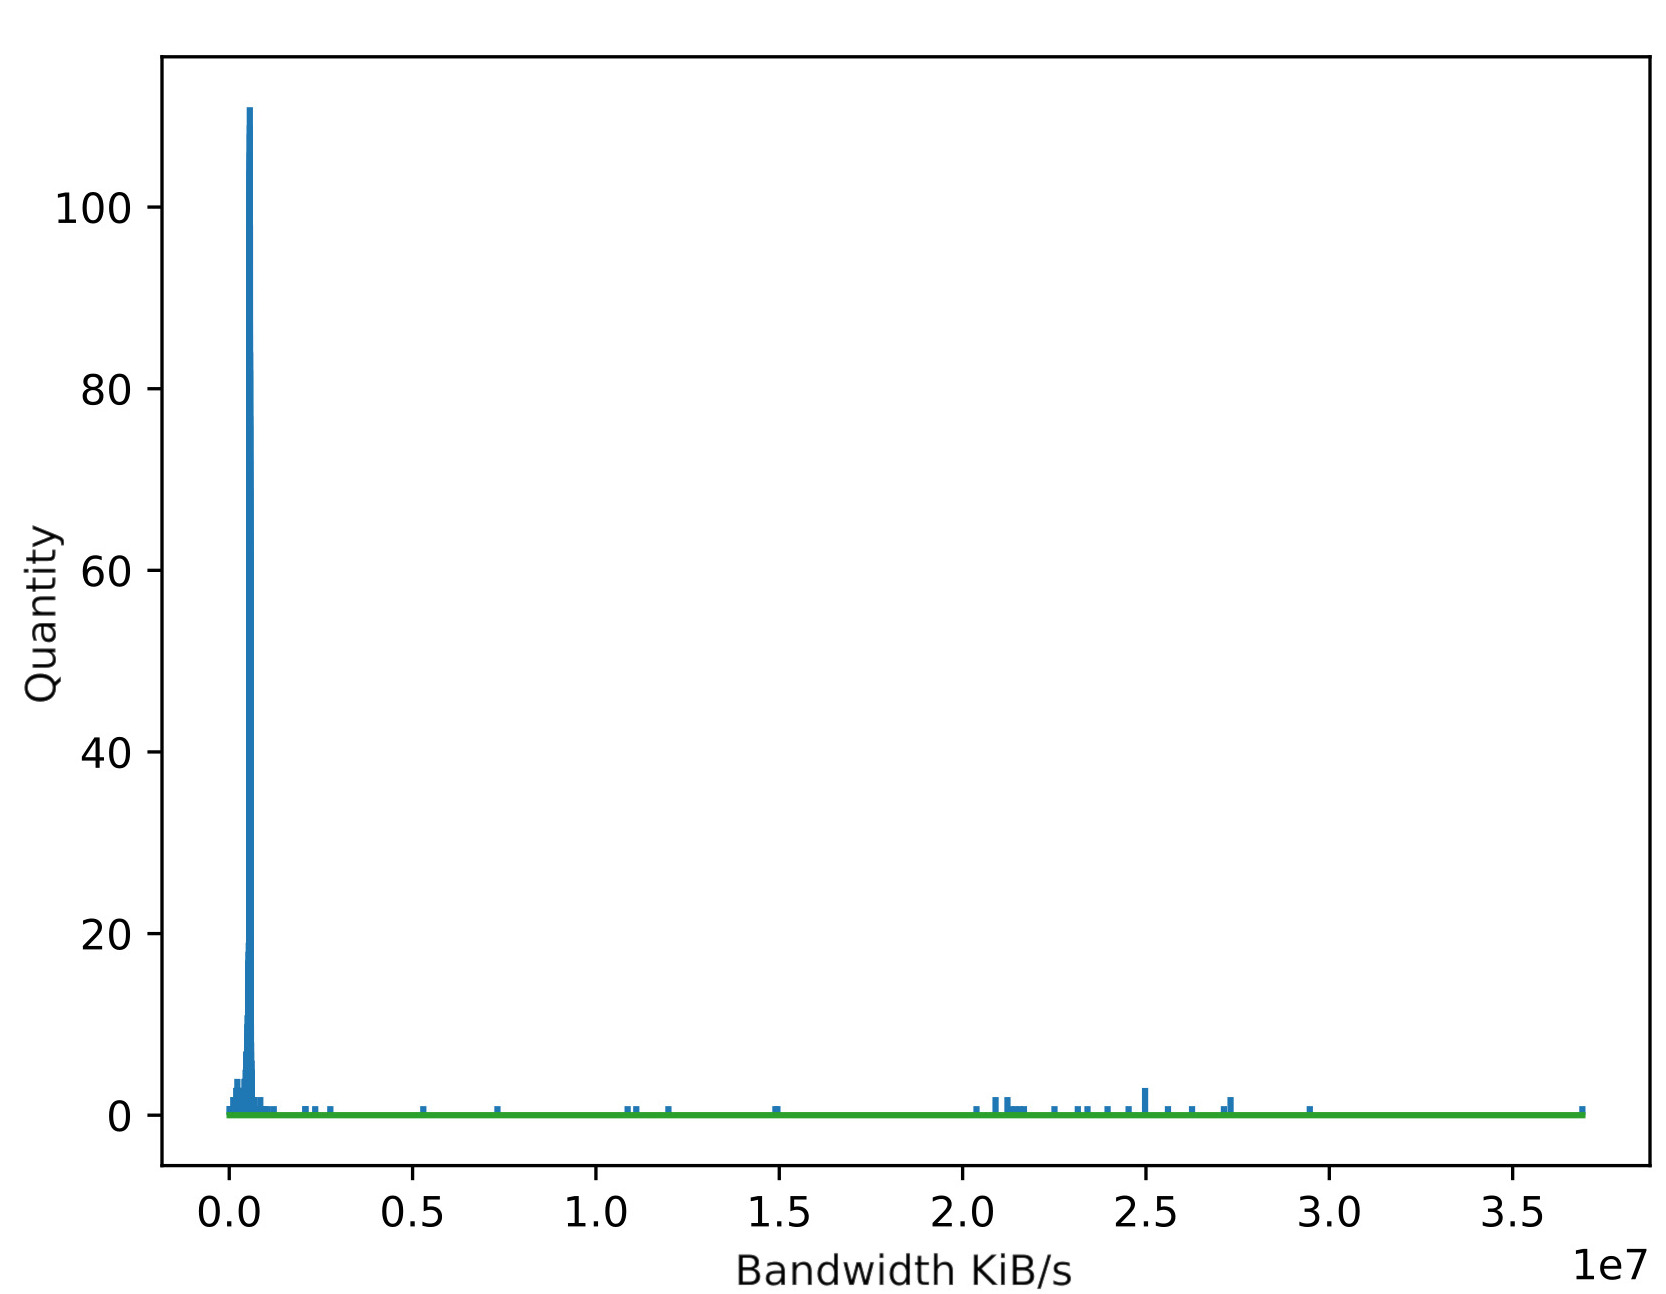
\includegraphics[width=5.5cm]{log_graph_bw_freq.jpg} }}%
    \qquad
    \subfloat[\centering Bandwidth per Msec]{{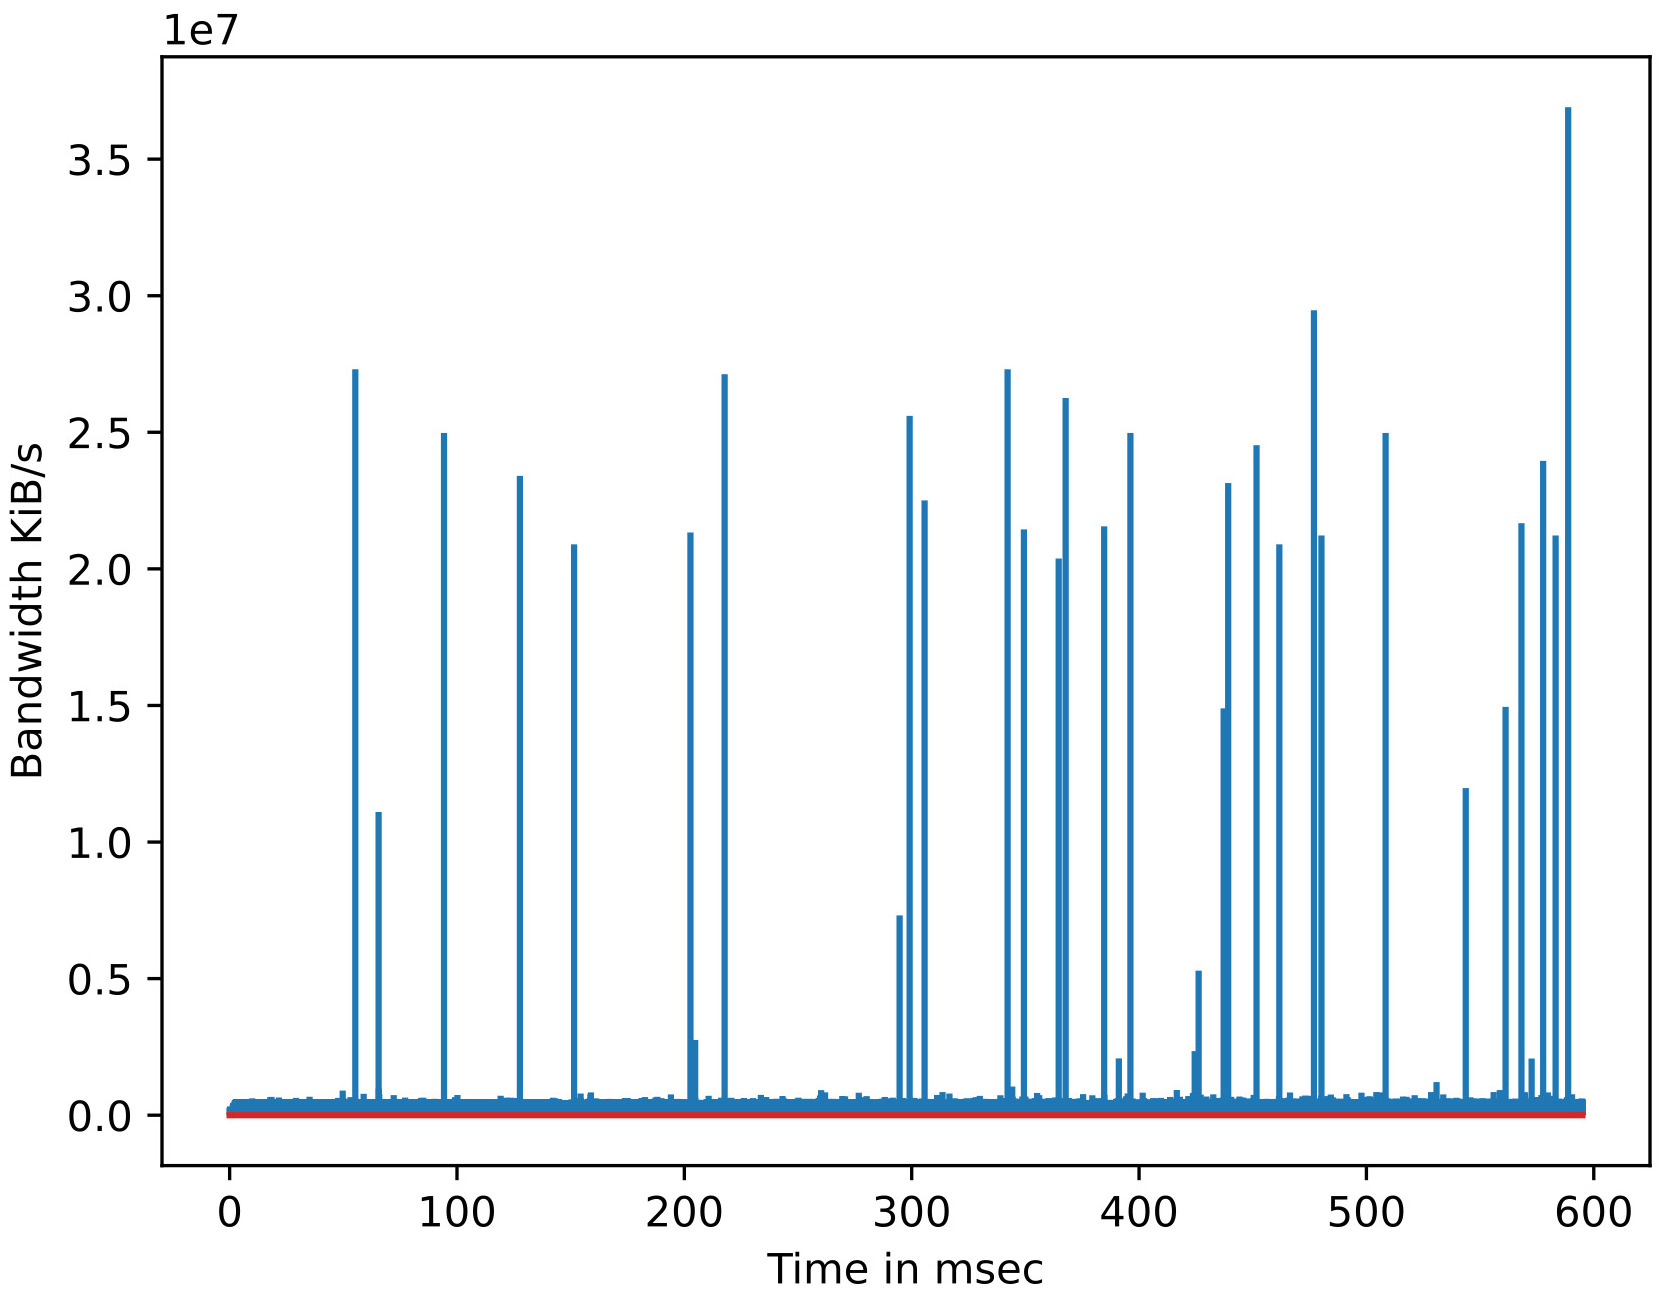
\includegraphics[width=5.5cm]{log_graph_time_to_bw.jpg} }}%
    \caption{fio Job: randread Bandbreite und Frequenz/Quantität}%
    \label{fig:log_graphs}%
\end{figure}


Der Computer, der verwendet wurde, hat ein 11th Gen Intel(R) Core(TM) i5-11400 @ 2.60GHz Prozessor und eine ADATA SWORDFISH 1TB SSD  als Datenträger.
Das kleine Tool diente mehr zum Einstieg. Die eigentliche Arbeit wird es sein, das Tool weiter auszubauen, das nicht nur veranschaulicht,
sondern auch den stationären Zustand berechnet.
Das Programm wird in Java geschrieben, da bereits entsprechende Vorkenntnisse vorhanden sind.
So soll mein Tool mit den Logdateien statistisch arbeiten.

\newpage
\section{Verwandte Arbeiten}
In der Arbeit von Barrett et al \cite{vmsHotandCold}. wurde tiefer auf Nichtdeterminismus von VMs eingegangen.
Dort wurde versucht, nicht-determinisitsche Faktoren so gering wie möglich zu halten, da sonst der stationäre Zustand nicht eintreten kann, auch wenn gleiche Workloads wiederholt durchlaufen werden. Auch  andere Hardware und Betriebssysteme haben wenig Einfluss auf die Zeit von Warmups. Li et al. \cite{9256518} arbeiteten ebenfalls mit VMs und testen die Performanz von diesen Maschinen mit verschiedener Anzahl an virtuellen CPUs. Und eine große Anzahl an VCPUs verbessert nicht zwingend die Performanz.
Georges et al \cite{10.1145/1297027.1297033}. verwendet statistische Methoden, wie Varianzanalyse und Tukey HSD, um eine akkurate Auswertung von den Experimenten berechnen zu können. Sie arbeiten ebenfalls mit VMs und VM Warmups.
Gründe für nicht-deterministisches Verhalten in VMs könnte Garbage Collection, Thread Scheduling oder auch Just-in-Time Compilation/Optimization sein \cite{stasticsInPerformance}.
AlGhmadi et al. erarbeiteten, wann Performanztests nach langem Testen redundant werden und wie viele Tests genug sind.

\section{Zeitplan}
Im ersten Teil der eigentlichen Arbeit werden die Grundlagen behandelt.
 Zuerst werden auf die Begrifflichkeiten wie Benchmarking, Warm-Up,
stationärer Zustand und fio-Tool erklärt. Nach den Erklärungen werden die Methodiken
der statististischen Analyse definiert, die das  Analysetool verwenden wird.
Im nächsten Kapitel werden die verwandten Arbeit beschrieben, die in
der Arbeit verwendet wurden. Im dritten Kapitel wird der Aufbau sowie die
Verwendung des Analystools eingegangen. Nach dem Analysetool, werden die
Experimente durchgeführt. Diese werden im vierten Kapitel für die Evaluierung
verwendet. Das letzte Kapitel ist die Zusammenfassung und Ausblick.
\newpage
\bibliography{cite}{}
\bibliographystyle{plain}
\end{document}